% =============================================================================
% CSE492 Thesis Defense Presentation
% On-Device American Sign Language Recognition
% Yusuf Kenan Akgun (20210702010) - Yeditepe University - 2026
%
% Compile:  pdflatex sunum && pdflatex sunum
% =============================================================================

\documentclass[aspectratio=169,11pt]{beamer}

% --- Theme ------------------------------------------------------------------
\usetheme{metropolis}
\usepackage{appendixnumberbeamer}

% --- Packages ---------------------------------------------------------------
\usepackage[utf8]{inputenc}
\usepackage[T1]{fontenc}
\usepackage{graphicx}
\usepackage{booktabs}
\usepackage{array}
\usepackage{tikz}
\usepackage{xcolor}
\usepackage{siunitx}
\usepackage{adjustbox}

\usetikzlibrary{shapes.geometric, arrows.meta, positioning, fit, backgrounds, calc}

\graphicspath{{../thesis/figures/}}

% --- Android app teal palette ----------------------------------------------
\definecolor{Teal}{HTML}{00897B}
\definecolor{TealDark}{HTML}{00695C}
\definecolor{TealCont}{HTML}{B2DFDB}
\definecolor{TealSoft}{HTML}{E0F2F1}
\definecolor{TealTint}{HTML}{F2F9F8}
\definecolor{TxtPri}{HTML}{101418}
\definecolor{TxtSec}{HTML}{5A6066}
\definecolor{CardBdr}{HTML}{ECEEF0}
\definecolor{Warn}{HTML}{B23A1F}

\setbeamercolor{frametitle}{bg=TealDark, fg=white}
\setbeamercolor{progress bar}{fg=Teal}
\setbeamercolor{alerted text}{fg=TealDark}
\setbeamercolor{normal text}{fg=TxtPri}
\setbeamercolor{itemize item}{fg=Teal}
\setbeamercolor{itemize subitem}{fg=Teal}

\setbeamertemplate{frametitle}{%
  \nointerlineskip%
  \begin{beamercolorbox}[wd=\paperwidth,sep=0pt,leftskip=0.7cm,rightskip=0.7cm]{frametitle}%
    \vskip6pt\strut\insertframetitle\strut\vskip6pt%
  \end{beamercolorbox}%
}

% --- Metadata ---------------------------------------------------------------
\title{On-Device American Sign Language Recognition}
\subtitle{Image- vs.\ Landmark-Based Approaches for Mobile Deployment}
\author{Yusuf Kenan Akg\"un\,\,\textperiodcentered\,\,20210702010}
\institute{Yeditepe University \,\,\textperiodcentered\,\, CSE492}
\date{2026}

\newcommand{\hl}[1]{\textcolor{TealDark}{\textbf{#1}}}
\newcommand{\hlb}[1]{\textcolor{Teal}{\textbf{#1}}}

% =============================================================================
\begin{document}

% --- SLIDE 1: COVER ---------------------------------------------------------
\begin{frame}[plain,noframenumbering]
  \begin{tikzpicture}[remember picture, overlay]
    \fill[TealDark] (current page.north west) rectangle ([yshift=-2.1cm]current page.north east);
    \fill[Teal] ([yshift=-2.1cm]current page.north west) rectangle ([yshift=-2.2cm]current page.north east);

    % Title
    \node[anchor=north west, text width=10.5cm, align=left, white]
      at ([xshift=0.9cm, yshift=-0.7cm]current page.north west)
      {\fontsize{19}{23}\selectfont\bfseries On-Device American\\Sign Language Recognition};

    % Subtitle (2 lines)
    \node[anchor=north west, text width=8.5cm, align=left, TxtPri]
      at ([xshift=0.9cm, yshift=-2.85cm]current page.north west)
      {\fontsize{11}{14}\selectfont\itshape Image- vs.\ Landmark-Based Approaches \\ for Mobile Deployment};

    % Divider
    \draw[Teal, line width=1.2pt]
      ([xshift=0.9cm, yshift=-4.05cm]current page.north west) --
      ([xshift=7.0cm, yshift=-4.05cm]current page.north west);

    % Author block
    \node[anchor=north west, text width=8.5cm, align=left, TxtPri]
      at ([xshift=0.9cm, yshift=-4.3cm]current page.north west)
      {\fontsize{10.5}{14}\selectfont
        \textbf{Yusuf Kenan Akg\"un} \,\textperiodcentered\, 20210702010 \\[2pt]
        Supervisor: \textbf{Bet\"ul Arslan} \\[2pt]
        Yeditepe University \,\textperiodcentered\, CSE492 \,\textperiodcentered\, 2026};

    % --- Three letter screenshots on the right --------------------------------
    \begin{scope}[shift={([xshift=-0.6cm, yshift=0.65cm]current page.south east)}]
      \node[anchor=south east] (sX)
        {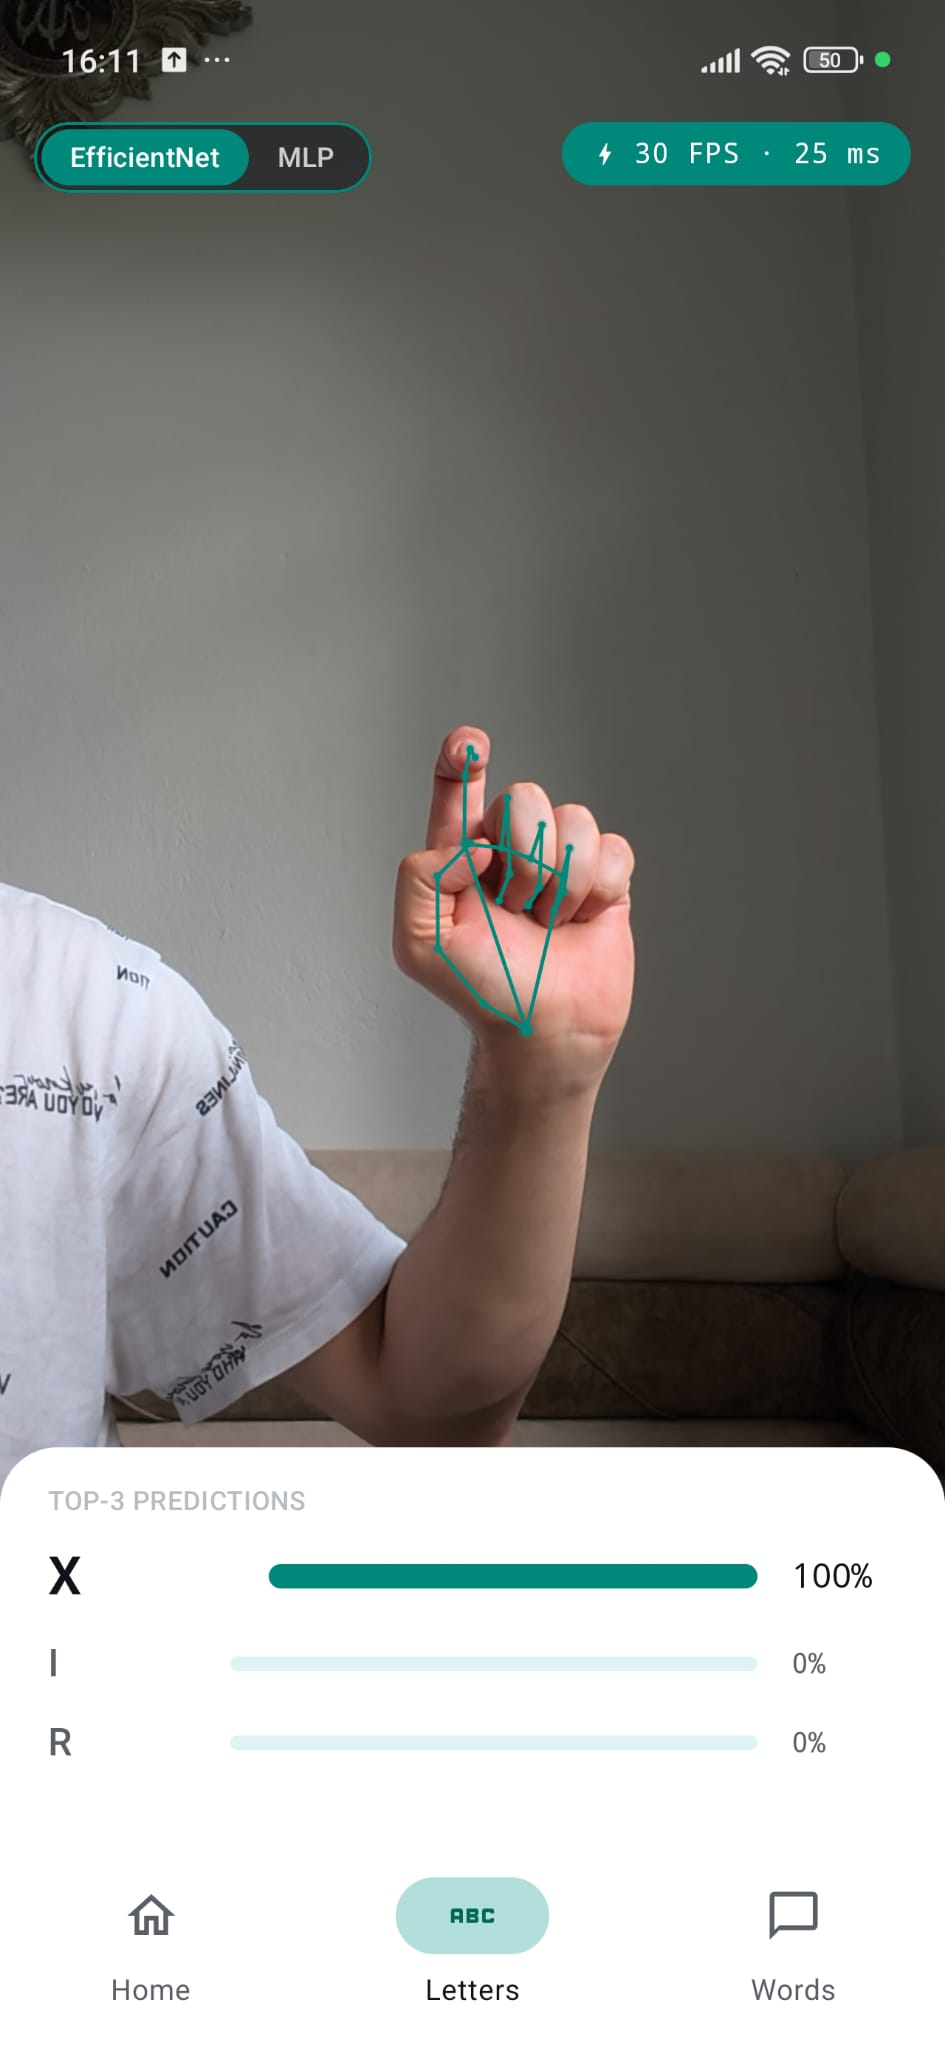
\includegraphics[height=3.7cm]{ui_xiaomi_X.jpg}};
      \node[anchor=south, font=\small\bfseries, TealDark]
        at ([yshift=0.02cm]sX.north) {X};

      \node[anchor=south east] (sB)
        at ([xshift=-0.15cm]sX.south west)
        {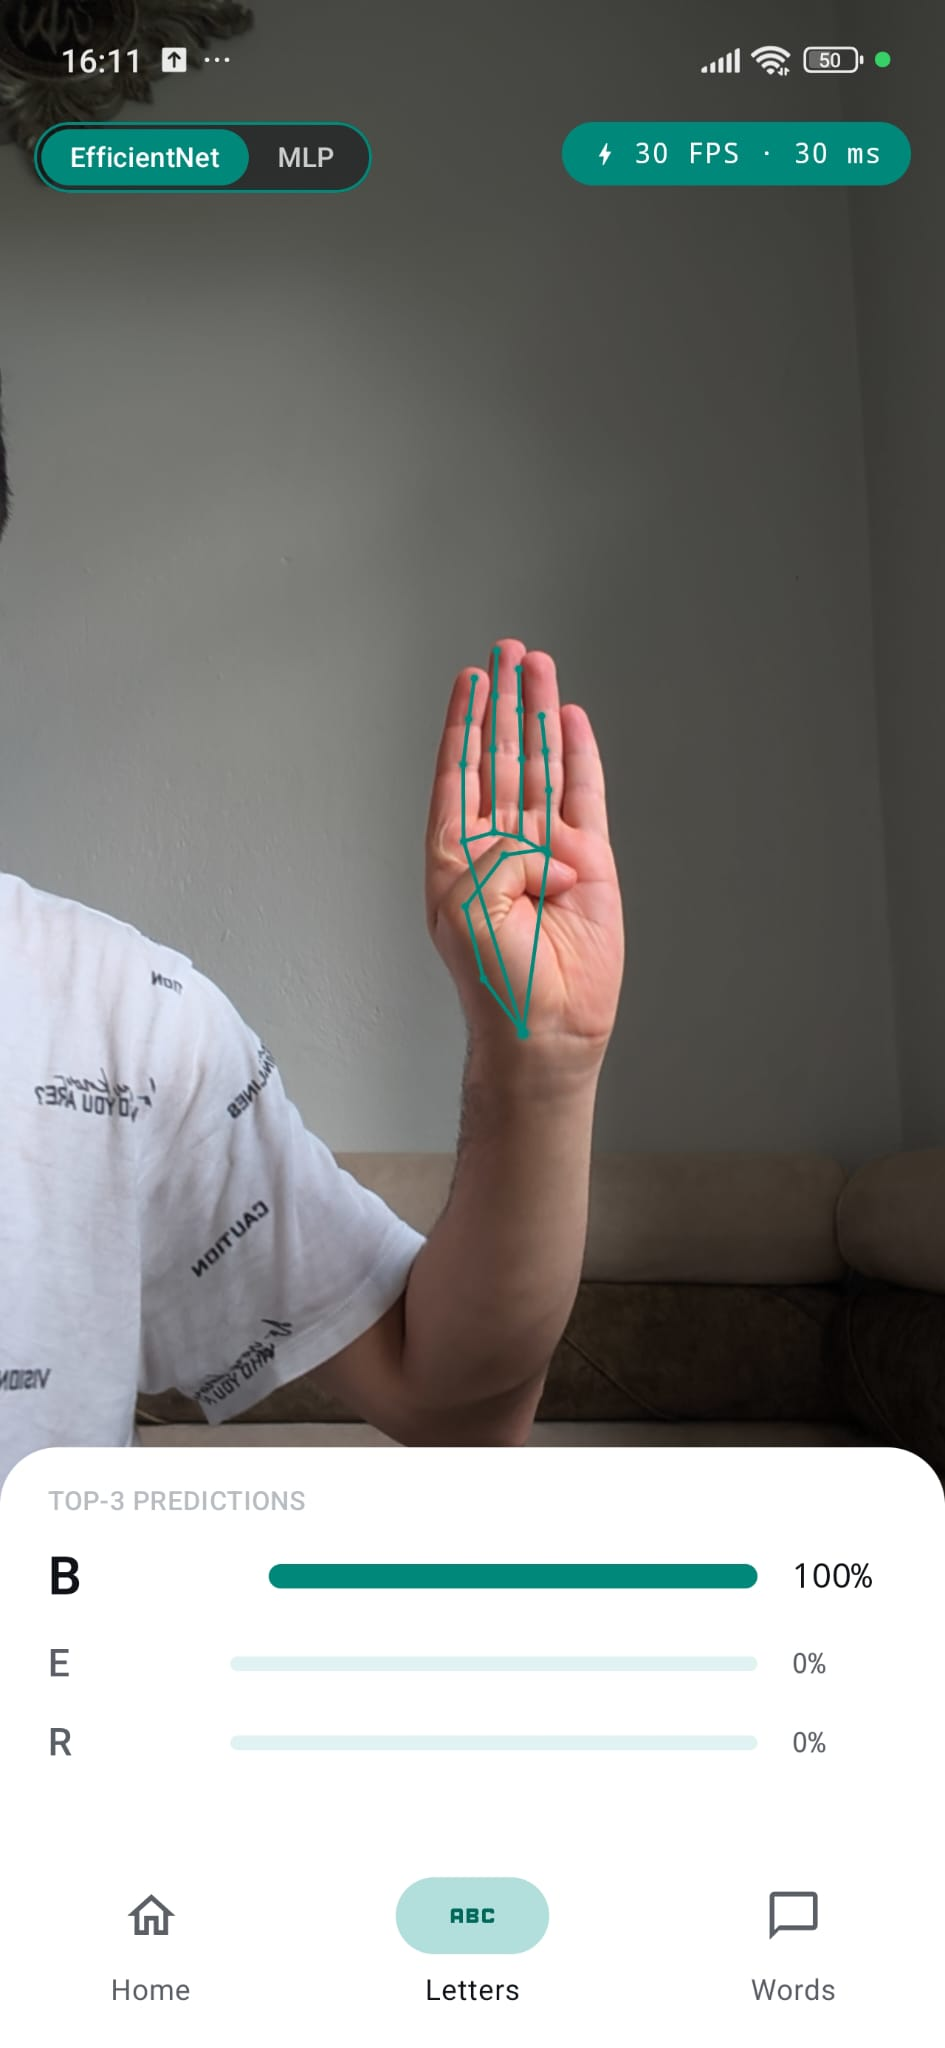
\includegraphics[height=3.7cm]{ui_xiaomi_B.jpg}};
      \node[anchor=south, font=\small\bfseries, TealDark]
        at ([yshift=0.02cm]sB.north) {B};

      \node[anchor=south east] (sA)
        at ([xshift=-0.15cm]sB.south west)
        {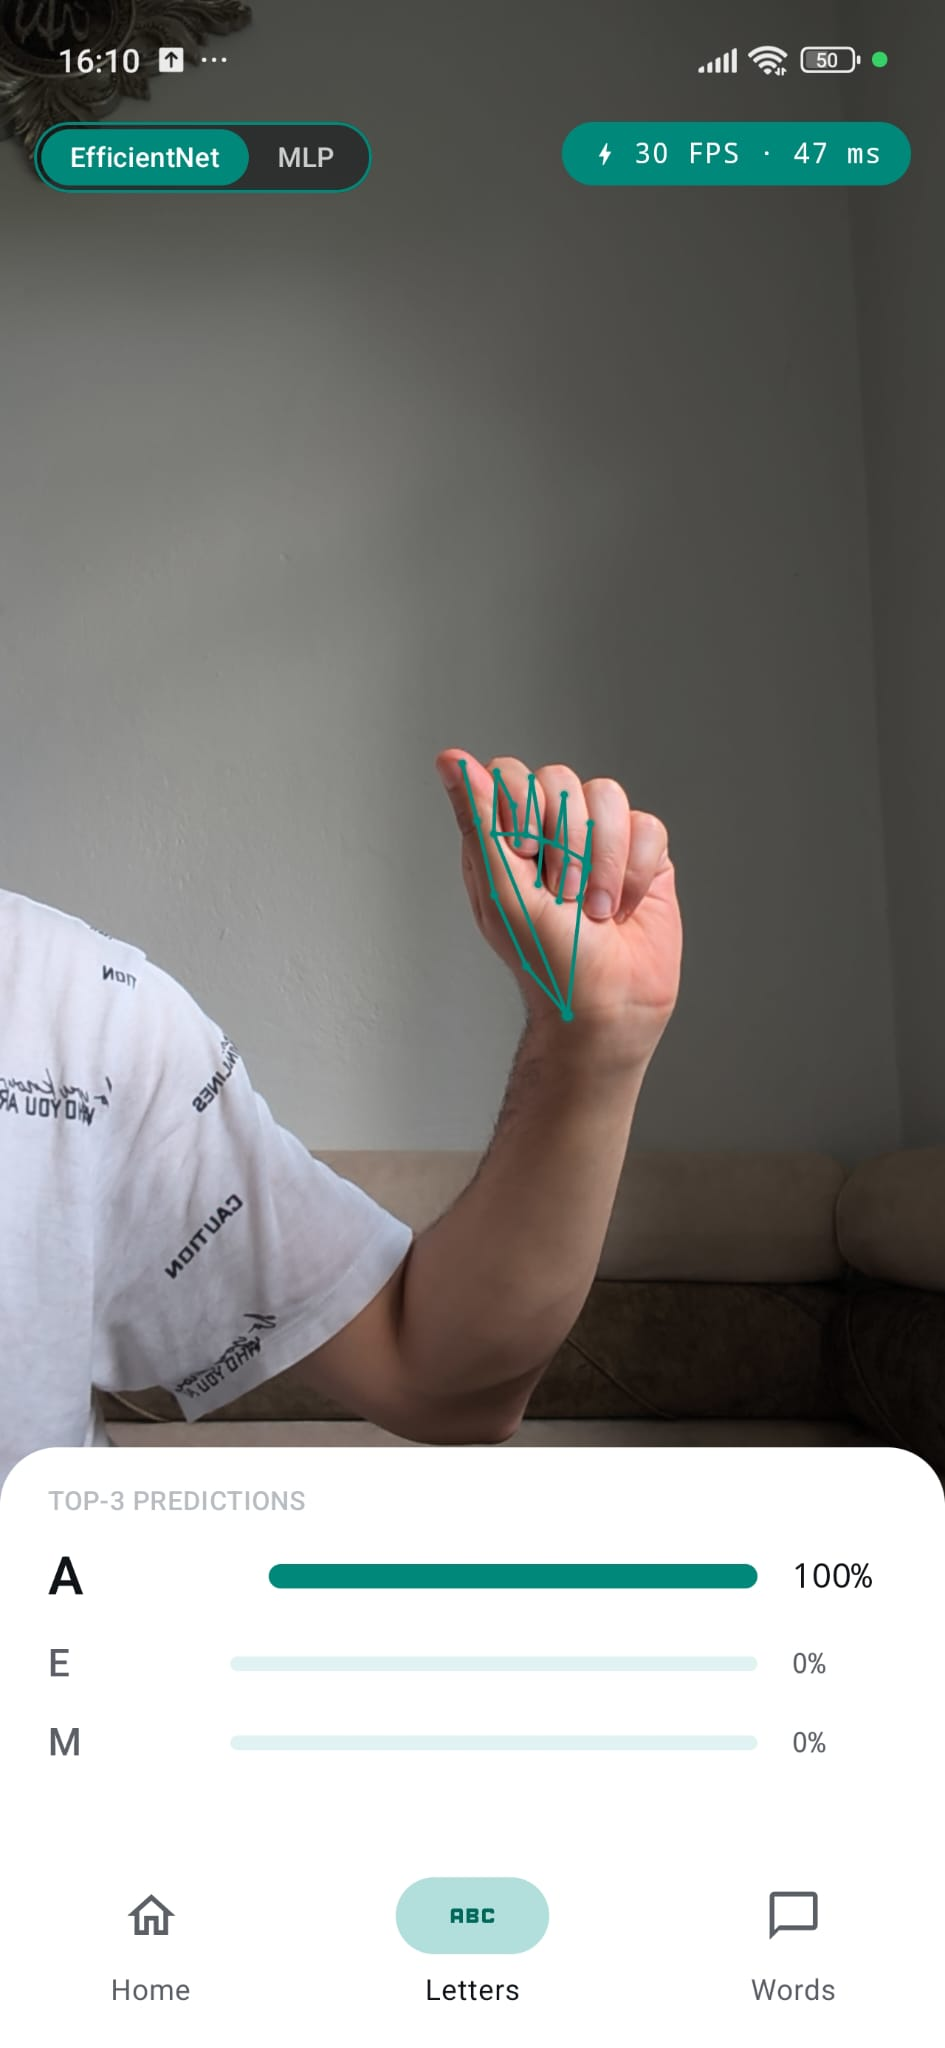
\includegraphics[height=3.7cm]{ui_xiaomi_A.jpg}};
      \node[anchor=south, font=\small\bfseries, TealDark]
        at ([yshift=0.02cm]sA.north) {A};
    \end{scope}

    \node[anchor=south east, TxtSec, font=\tiny\itshape]
      at ([xshift=-0.7cm, yshift=0.35cm]current page.south east)
      {Letters tab \,\textperiodcentered\, landmark overlay};
  \end{tikzpicture}
\end{frame}

% --- SLIDE 2: INTRODUCTION --------------------------------------------------
\begin{frame}{Introduction}
  \begin{center}
    {\normalsize\bfseries\color{TealDark}The Gap:} \hlb{Accurate on a server} \,$\neq$\, \hl{usable on a phone}
  \end{center}

  \vspace{0.1cm}
  \begin{columns}[T,onlytextwidth]
    \column{0.50\textwidth}
      \small
      \begin{itemize}\setlength{\itemsep}{6pt}
        \item Sign language remains \hl{underserved} by consumer technology
        \item Literature optimises offline \hl{accuracy}, rarely \hl{deployability}
        \item Two complementary tasks:
        \begin{itemize}\setlength{\itemsep}{2pt}
          \item[\textbullet] \textbf{Letters} --- 29 static classes
          \item[\textbullet] \textbf{Words} --- WLASL-100, temporal
        \end{itemize}
        \item Hard constraint: \hl{100\,\% on-device}, no server
      \end{itemize}

    \column{0.48\textwidth}
      \centering
      \scriptsize\bfseries\color{TxtPri} Word recognition flow \,\textperiodcentered\, ``drink''\\[3pt]
      \begin{tikzpicture}[
          node distance=0.20cm,
          ss/.style={draw=CardBdr, line width=0.6pt, rounded corners=3pt, inner sep=1.5pt},
          stagelbl/.style={font=\tiny\bfseries, TealDark, align=center}
        ]
        \node[ss] (s1) {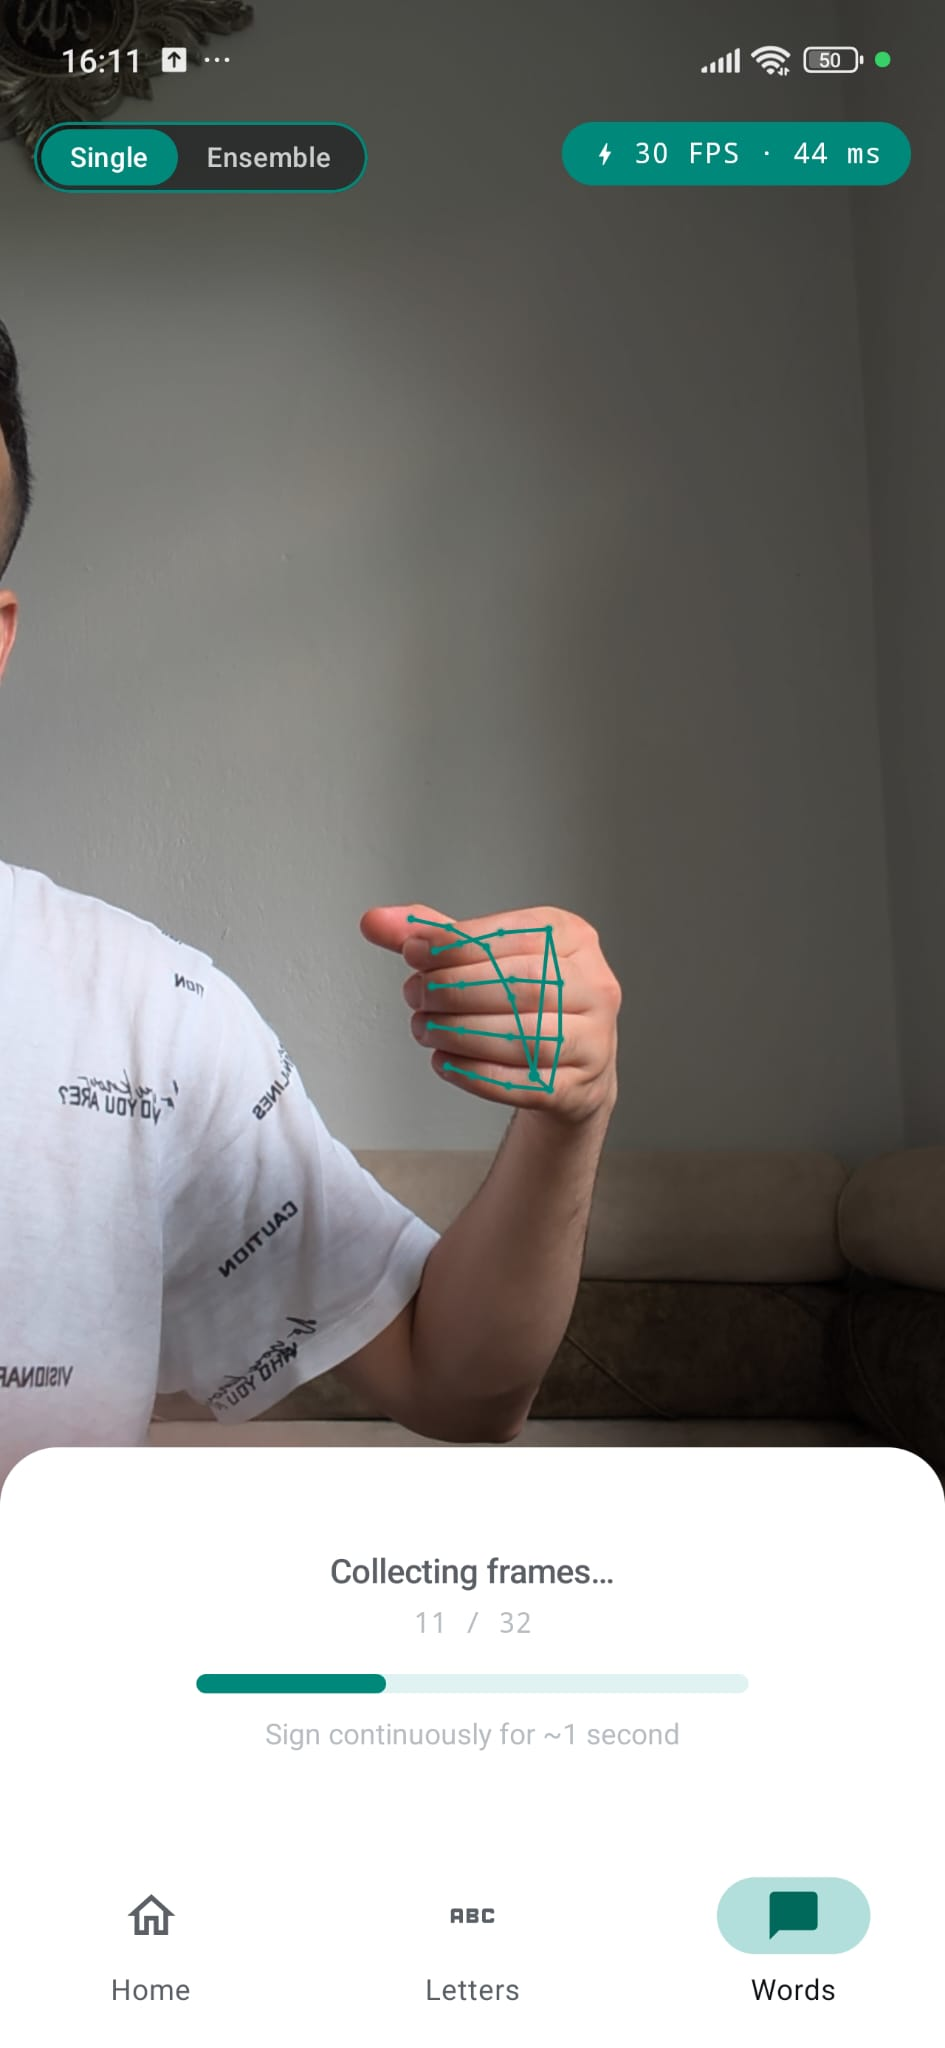
\includegraphics[height=3.4cm]{ui_drink_collect.jpg}};
        \node[ss, right=of s1] (s2) {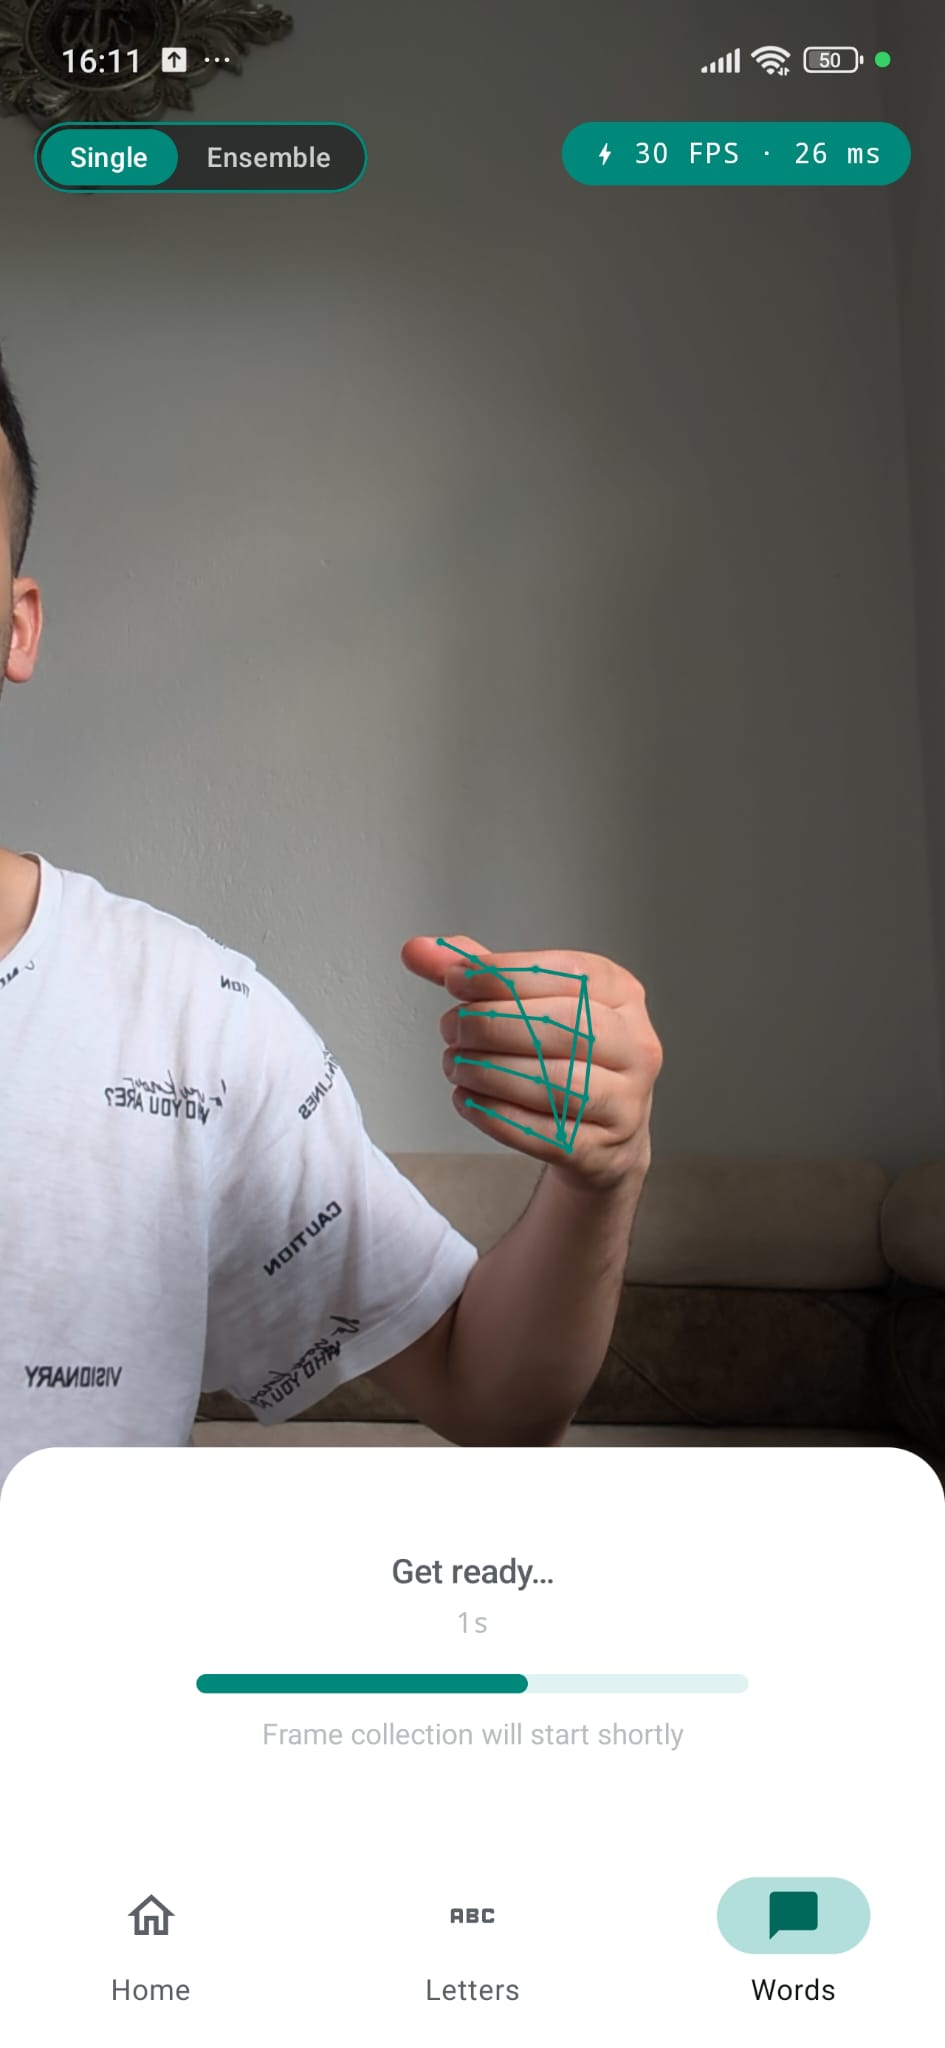
\includegraphics[height=3.4cm]{ui_drink_ready.jpg}};
        \node[ss, right=of s2] (s3) {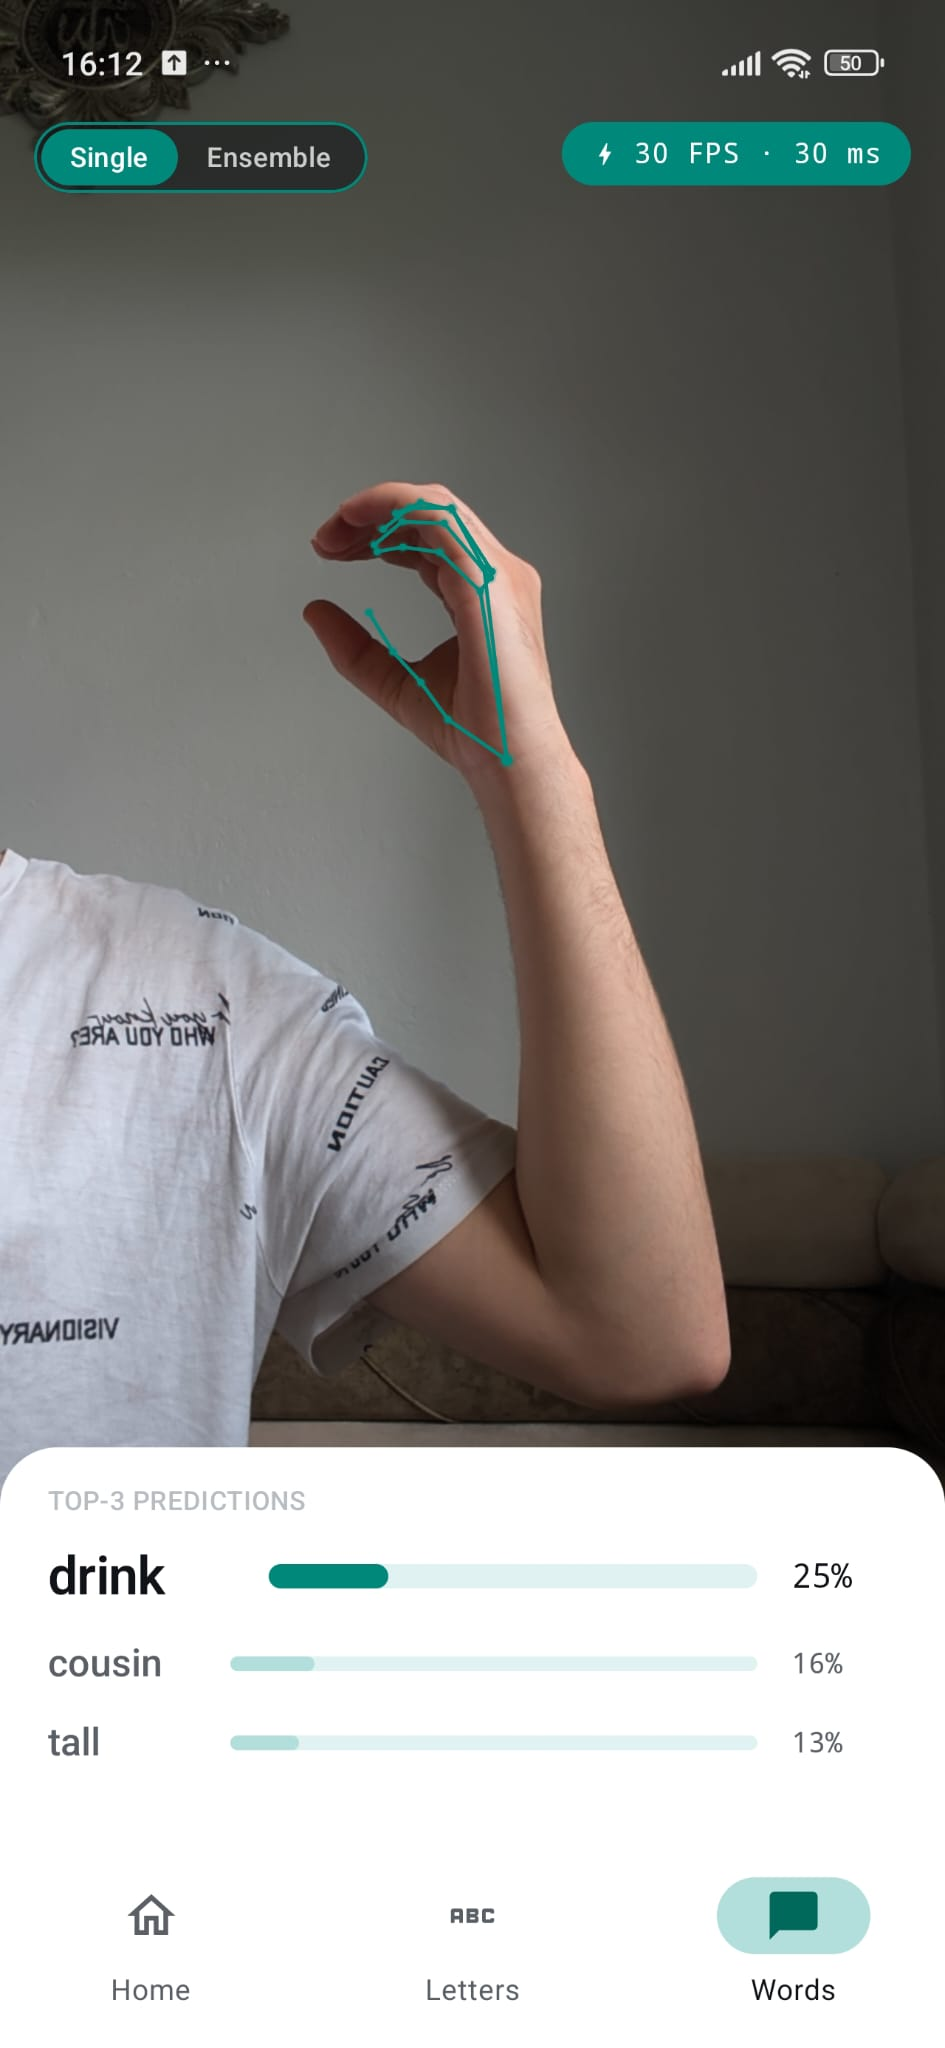
\includegraphics[height=3.4cm]{ui_drink_result.jpg}};

        \node[stagelbl, below=2pt of s1] {Collect};
        \node[stagelbl, below=2pt of s2] {Ready};
        \node[stagelbl, below=2pt of s3] {Result};

        % Arrows between stages
        \draw[-Stealth, Teal, line width=0.7pt]
          ([yshift=-0.15cm]s1.east) -- ([yshift=-0.15cm]s2.west);
        \draw[-Stealth, Teal, line width=0.7pt]
          ([yshift=-0.15cm]s2.east) -- ([yshift=-0.15cm]s3.west);
      \end{tikzpicture}\\[2pt]
      {\tiny\itshape\color{TxtSec} 32-frame window \,\textperiodcentered\, BiLSTM latches top-1}
  \end{columns}
\end{frame}

% --- SLIDE 3: SYSTEM ARCHITECTURE -------------------------------------------
\begin{frame}{System Architecture}
  \begin{center}
    {\normalsize One artefact bridges two worlds: the \hl{TFLite checkpoint}}
  \end{center}

  \vspace{0.05cm}
  \begin{center}
  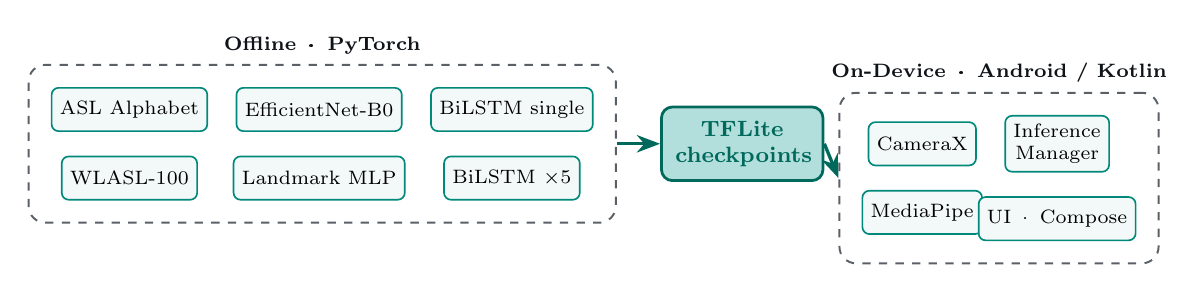
\begin{tikzpicture}[
      node distance=0.30cm and 0.35cm,
      block/.style={draw=Teal, fill=TealTint, rounded corners=2.5pt, line width=0.6pt,
                    minimum height=0.55cm, font=\scriptsize, inner sep=3pt, align=center},
      grp/.style={draw=TxtSec, dashed, rounded corners=6pt, line width=0.7pt,
                  inner sep=8pt},
      bridge/.style={draw=TealDark, fill=TealCont, rounded corners=4pt,
                     line width=1.0pt, minimum height=0.9cm, font=\footnotesize\bfseries,
                     inner sep=5pt, align=center, text=TealDark},
      bigarrow/.style={-Stealth, line width=1.2pt, TealDark},
      grouptitle/.style={font=\bfseries\scriptsize, TxtPri}
    ]

    \node[block]                  (ds)  {ASL Alphabet};
    \node[block, below=of ds]     (wl)  {WLASL-100};
    \node[block, right=of ds]     (cnn) {EfficientNet-B0};
    \node[block, below=of cnn]    (mlp) {Landmark MLP};
    \node[block, right=of cnn]    (lstm){BiLSTM single};
    \node[block, below=of lstm]   (ens) {BiLSTM $\times$5};

    \node[grp, fit=(ds)(wl)(cnn)(mlp)(lstm)(ens),
          label={[grouptitle]above:Offline \,\textperiodcentered\, PyTorch}] (offline) {};

    \node[bridge, right=0.55cm of offline, text width=1.7cm] (tfl)
      {TFLite \\ checkpoints};

    \node[block, right=0.55cm of tfl]  (cam) {CameraX};
    \node[block, below=of cam]         (mp)  {MediaPipe};
    \node[block, right=of cam]         (inf) {Inference \\ Manager};
    \node[block, below=of inf]         (ui)  {UI \,\textperiodcentered\, Compose};

    \node[grp, fit=(cam)(mp)(inf)(ui),
          label={[grouptitle]above:On-Device \,\textperiodcentered\, Android / Kotlin}] (ondev) {};

    \draw[bigarrow] (offline.east) -- (tfl.west);
    \draw[bigarrow] (tfl.east) -- (ondev.west);

  \end{tikzpicture}
  \end{center}

  \vspace{0.05cm}
  \begin{center}
    \footnotesize\itshape \textcolor{TxtSec}{Four models \,\textperiodcentered\, two datasets \,\textperiodcentered\, one Android app}
  \end{center}
\end{frame}

% --- SLIDE 4: IMPLEMENTATION ------------------------------------------------
\begin{frame}{Implementation}
  \begin{center}
    {\normalsize \hl{4 models} \,\textperiodcentered\, \hl{2 datasets} \,\textperiodcentered\, \hl{1 app}}
  \end{center}

  \vspace{0.10cm}
  \begin{columns}[T,onlytextwidth]
    \column{0.50\textwidth}
      \scriptsize\bfseries\color{Teal}Models \,\textperiodcentered\, two tasks\\[3pt]
      \scriptsize

      \textbf{\color{TealDark}Letters task}\\[1pt]
      \begin{itemize}\setlength{\itemsep}{1pt}\setlength{\topsep}{0pt}\setlength{\leftskip}{-8pt}
        \item \textbf{EfficientNet-B0} --- $224^2$ RGB, ImageNet pretrain
        \item \textbf{Landmark MLP} --- 63-D MediaPipe pose
      \end{itemize}
      \vspace{2pt}
      \textbf{\color{TealDark}Words task}\\[1pt]
      \begin{itemize}\setlength{\itemsep}{1pt}\setlength{\topsep}{0pt}\setlength{\leftskip}{-8pt}
        \item \textbf{BiLSTM} --- $128{\times}32$ two-hand landmark stream
        \item \textbf{BiLSTM $\times 5$ ens.} --- 5-seed logit averaging
      \end{itemize}

      \vspace{0.12cm}
      \scriptsize\bfseries\color{Teal}Datasets\\[2pt]
      \scriptsize
      \begin{itemize}\setlength{\itemsep}{1pt}\setlength{\topsep}{0pt}\setlength{\leftskip}{-8pt}
        \item \textbf{ASL Alphabet} --- 87{,}000 images \,\textperiodcentered\, 29 classes
        \item \textbf{WLASL-100} --- 1{,}013 $\rightarrow$ \hl{1{,}465 clips} \\
              {\tiny yt-dlp recovery, \hl{+44\,\%} over Kaggle baseline}
      \end{itemize}

    \column{0.48\textwidth}
      \scriptsize\bfseries\color{Teal}Ablation Technique\\[2pt]
      \scriptsize
      Forward-additive 9-step protocol on WLASL-100 val; each pillar isolated to measure its incremental gain.\\[4pt]

      \textbf{\color{TealDark}Four cumulative pillars}\\[1pt]
      \begin{itemize}\setlength{\itemsep}{1pt}\setlength{\topsep}{0pt}\setlength{\leftskip}{-8pt}
        \item \textbf{Data engineering} --- yt-dlp recovery, re-balancing
        \item \textbf{Extraction} --- two-hand pose, hand-crop norm.
        \item \textbf{Training recipe} --- aug.\ + mixup + sampling
        \item \textbf{Ensemble} --- 5-seed logit averaging
      \end{itemize}
      \vspace{3pt}

      
\begin{tikzpicture}
        \node[draw=TealDark, fill=TealSoft, rounded corners=4pt,
              line width=1.0pt, text width=5.4cm, align=center, inner sep=4pt]
          {\scriptsize\bfseries\color{TxtPri} Data engineering = \color{TealDark}largest lever
           \color{TxtPri}($+16$\,pp).};
      \end{tikzpicture}
  \end{columns}
\end{frame}

% --- SLIDE 5: TESTS & RESULTS -----------------------------------------------
\begin{frame}{Tests \& Results}
  \begin{center}
    {\normalsize The offline ranking \hl{inverts} on a budget phone}
  \end{center}

  \vspace{0.05cm}
  \begin{columns}[T,onlytextwidth]
    \column{0.52\textwidth}
      \footnotesize\bfseries\color{Teal}Letters \,\textperiodcentered\, Top-1 accuracy\\[2pt]
      \small
      \renewcommand{\arraystretch}{1.10}
      \resizebox{\linewidth}{!}{%
      \begin{tabular}{@{}l c c c@{}}
        \toprule
                       & \textbf{Offline} & \textbf{TECNO} & \textbf{Xiaomi} \\
        \midrule
        EfficientNet-B0 & 100.0\,\%        & \textcolor{Warn}{\textbf{92.9\,\%}}      & 100.0\,\% \\
        Landmark MLP    & 99.4\,\%         & \hl{100.0\,\%} & \hl{100.0\,\%} \\
        \bottomrule
      \end{tabular}}\\[2pt]
      {\scriptsize\itshape\color{TxtSec}
        Ships in \hl{0.24\,MB} vs.\ \hlb{15.71\,MB} (EfficientNet).}

      \vspace{0.04cm}
      \scriptsize\bfseries\color{Teal}Words \,\textperiodcentered\, WLASL-100\\[1pt]
      \scriptsize
      \renewcommand{\arraystretch}{1.05}
      \begin{tabular}{@{}l c c c@{}}
        \toprule
                              & \textbf{Offline}     & \multicolumn{2}{c}{\textbf{Xiaomi}} \\
        \cmidrule(lr){2-2}\cmidrule(lr){3-4}
                              & \textbf{Top-1}       & \textbf{Top-1}   & \textbf{Top-3} \\
        \midrule
        BiLSTM (single)       & 52.1\,\%             & 38.0\,\%         & 71.0\,\% \\
        BiLSTM $\times 5$ ens. & 56.2\,\%             & 49.0\,\%         & \hl{72.0\,\%} \\
        \bottomrule
      \end{tabular}\\[3pt]
      {\scriptsize\itshape\color{TxtSec} Ensemble clears 40\,\% bar; Top-3 $\sim$72\,\% --- usable UX.}

    \column{0.46\textwidth}
      \scriptsize\bfseries\color{Teal}Throughput \,\textperiodcentered\, latency (ms) \,/\, FPS\\[2pt]
      \footnotesize
      \renewcommand{\arraystretch}{1.00}
      \begin{tabular}{@{}l c c@{}}
        \toprule
                            & \textbf{Xiaomi 15T Pro} & \textbf{TECNO 20C} \\
        \midrule
        EfficientNet-B0     & 35\,/\,30   & 203\,/\,21  \\
        Landmark MLP        & 19\,/\,30   & 22\,/\,24   \\
        BiLSTM (single)     & 32\,/\,30   & \textcolor{Warn}{\textbf{202\,/\,22}} \\
        BiLSTM $\times 5$   & 80\,/\,30   & \textcolor{Warn}{\textbf{665\,/\,17}} \\
        \bottomrule
      \end{tabular}\\[1pt]
      {\scriptsize\itshape\color{TxtSec}
        TECNO word models \textcolor{Warn}{not interactive}.}

      \vspace{0.02cm}
      \begin{center}
      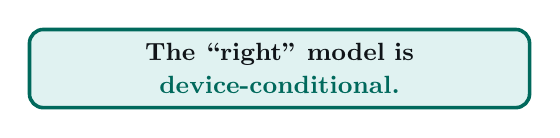
\begin{tikzpicture}
        \node[draw=TealDark, fill=TealSoft, rounded corners=5pt,
              line width=1.3pt, text width=6.0cm, align=center, inner sep=5pt]
          {\small\bfseries\color{TxtPri} The ``right'' model is \color{TealDark}device-conditional.};
      \end{tikzpicture}
      \end{center}
  \end{columns}
\end{frame}

\end{document}
